
%\VignetteIndexEntry{Follow-up data with R and Epi}
\documentclass[a4paper,dvipsnames,twoside,12pt]{report}

\newcommand{\Title}{Follow-up data with \R\ and \texttt{Epi}}
\newcommand{\Tit}{Follow-up}
\newcommand{\Version}{\ }
\newcommand{\Dates}{December 2017}
\newcommand{\Where}{SDCC}
\newcommand{\Homepage}{\url{http://bendixcarstensen.com/} }
\newcommand{\Faculty}{\begin{tabular}{rl}
Bendix Carstensen
  & Steno Diabetes Center, Gentofte, Denmark\\
  & {\small \& Department of Biostatistics,
               University of Copenhagen} \\
  & \texttt{b@bxc.dk} \\
  & \url{http://BendixCarstensen.com} \\[1em]
                      \end{tabular}}

%----------------------------------------------------------------------
% Packages
%\usepackage[inline]{showlabels}
%\usepackage[latin1]{inputenc}
\usepackage[utf8]{inputenc}
\usepackage[T1]{fontenc}
\usepackage[english]{babel}
\usepackage[font=it,labelfont=normalfont]{caption}
\usepackage[colorlinks,urlcolor=blue,linkcolor=red,citecolor=Maroon]{hyperref}
\usepackage[dvipsnames]{xcolor}
\usepackage[super]{nth}
% \usepackage[retainorgcmds]{IEEEtrantools}
\usepackage[noae]{Sweave}
\usepackage[ae,hyper]{Rd}
% \usepackage[noae]{C:/util/R/R-4.2.0/share/texmf/tex/latex/Sweave}
% \usepackage{C:/util/R/R-4.2.0/share/texmf/tex/latex/Rd}
\usepackage{makeidx,floatflt,amsmath,amsfonts,amsbsy,enumitem,dcolumn,needspace}
\usepackage{ifthen,calc,eso-pic,everyshi}
\usepackage{booktabs,longtable,rotating,graphicx,subfig}
\usepackage{pdfpages,verbatim,fancyhdr,datetime,afterpage}
\usepackage[abspath]{currfile}
% \usepackage{times}
\renewcommand{\textfraction}{0.0}
\renewcommand{\topfraction}{1.0}
\renewcommand{\bottomfraction}{1.0}
\renewcommand{\floatpagefraction}{0.9}
\definecolor{blaa}{RGB}{99,99,255}
\DeclareGraphicsExtensions{.png,.pdf,.jpg}
% Make the Sweave output nicer (slightly mor compact)
\DefineVerbatimEnvironment{Sinput}{Verbatim}{fontsize=\small,fontshape=sl,formatcom=\color{BlueViolet}}
\DefineVerbatimEnvironment{Soutput}{Verbatim}{fontsize=\small,formatcom=\color{Sepia},xleftmargin=0em}
\DefineVerbatimEnvironment{Scode}{Verbatim}{fontsize=\small}
\fvset{listparameters={\setlength{\topsep}{-0.1ex}}}
\renewenvironment{Schunk}%
{\renewcommand{\baselinestretch}{0.87} \vspace{\topsep}}%
{\renewcommand{\baselinestretch}{1.00} \vspace{\topsep}}
% \renewenvironment{knitrout}
% {\renewcommand{\baselinestretch}{0.87}}
% {\renewcommand{\baselinestretch}{1.00}}
% This is a file of useful extra commands snatched from
% Michael Hills, David Clayton, Bendix Carstensen & Esa Laara.
%

% Commands to draw observation lines on follow-up diagrams
%
% Horizontal lines
%
\providecommand{\hfail}[1]{\begin{picture}(250,5)
      \put(0,0){\line(1,0){#1}}
      \put(#1,0){\circle*{5}}
   \end{picture}}

\providecommand{\hcens}[1]{\begin{picture}(250,5)
      \put(0,0){\line(1,0){#1}}
      \put(#1,0){\line(0,1){2.5}}
      \put(#1,0){\line(0,-1){2.5}}
   \end{picture}}

%
% Diagonals for Lexis diagrams
%
\providecommand{\dfail}[1]{\begin{picture}(250,250)
      \put(0,0){\line(1,1){#1}}
      \put(#1,#1){\circle*{5}}
   \end{picture}}

\providecommand{\dcens}[1]{\begin{picture}(250,250)
      \put(0,0){\line(1,1){#1}}
%      \put(#1,#1){\line(0,1){2.5}}
%      \put(#1,#1){\line(0,-1){2.5}}
% BxC Changed this to an open circle instead of a line
      \put(#1,#1){\circle{5}}
   \end{picture}}

%
% Horizontal range diagrams
%
\providecommand{\hrange}[1]{\begin{picture}(200,5)
     \put(0,0){\circle*{5}}
     \put(0,0){\line(1,0){#1}}
     \put(0,0){\line(-1,0){#1}}
   \end{picture}}

%
% Tree drawing
%
\providecommand{\Tree}[3]{\setlength{\unitlength}{#1\unitlength}\begin{picture}(0,0)
   \put(0,0){\line(3, 2){1}}
   \put(0,0){\line(3,-2){1}}
   \put(0.81, 0.54){\makebox(0,0)[br]{\footnotesize #2\ }}
   \put(0.81,-0.54){\makebox(0,0)[tr]{\footnotesize #3\ }}
\end{picture}}

\providecommand{\Wtree}[3]{\setlength{\unitlength}{#1\unitlength}\begin{picture}(0,0)
   \put(0,0){\line(1, 1){1}}
   \put(0,0){\line(1,-1){1}}
   \put(0.8,0.8){\makebox(0,0)[br]{\footnotesize #2\ }}
   \put(0.8,-0.8){\makebox(0,0)[tr]{\footnotesize #3\ }}
\end{picture}}

\providecommand{\Ntree}[3]{\setlength{\unitlength}{#1\unitlength}\begin{picture}(0,0)
   \put(0,0){\line(2, 1){1}}
   \put(0,0){\line(2,-1){1}}
   \put(0.8,0.4){\makebox(0,0)[br]{\footnotesize #2\ }}
   \put(0.8,-0.4){\makebox(0,0)[tr]{\footnotesize #3\ }}
\end{picture}}

\providecommand{\Nutree}[3]{\setlength{\unitlength}{#1\unitlength}\begin{picture}(0,0)
   \put(0,0){\line(2, 1){#1}}
   \put(0,0){\line(2,-1){#1}}
   \put(0.8,0.4){\makebox(0,0)[br]{#2\ }}
   \put(0.8,-0.4){\makebox(0,0)[tr]{#3\ }}
\end{picture}}

%
% Tree drawing
%
\providecommand{\tree}[3]{\setlength{\unitlength}{#1}\begin{picture}(0,0)
   \put(0,0){\line(3,2){1}}
   \put(0,0){\line(3,-2){1}}
   \put(0.81,0.54){\makebox(0,0)[br]{\footnotesize #2\ }}
   \put(0.81,-0.54){\makebox(0,0)[tr]{\footnotesize #3\ }}
\end{picture}}

\providecommand{\wtree}[3]{\setlength{\unitlength}{#1}\begin{picture}(0,0)
   \put(0,0){\line(1,1){1}}
   \put(0,0){\line(1,-1){1}}
   \put(0.8,0.8){\makebox(0,0)[br]{\footnotesize #2\ }}
   \put(0.8,-0.8){\makebox(0,0)[tr]{\footnotesize #3\ }}
\end{picture}}

\providecommand{\ntree}[3]{\setlength{\unitlength}{#1}\begin{picture}(0,0)
   \put(0,0){\line(2,1){1}}
   \put(0,0){\line(2,-1){1}}
   \put(0.8,0.4){\makebox(0,0)[br]{\footnotesize #2\ }}
   \put(0.8,-0.4){\makebox(0,0)[tr]{\footnotesize #3\ }}
\end{picture}}

\providecommand{\nutree}[3]{\begin{picture}(0,0)
   \put(0,0){\line(2,1){#1}}
   \put(0,0){\line(2,-1){#1}}
   \put(0.8,0.4){\makebox(0,0)[br]{#2\ }}
   \put(0.8,-0.4){\makebox(0,0)[tr]{#3\ }}
\end{picture}}

%
% Other commands
%
\providecommand{\ip}[2]{\langle #1 \vert #2 \rangle} 
\providecommand{\I}{\text{\rm gI}}
\providecommand{\prob}[0]{\text{\rm Pr}}
\providecommand{\nhy}[0]{_{\oslash}}
\providecommand{\true}[0]{_{\text{\rm \tiny T}}}
\providecommand{\hyp}[0]{_{\text{\rm \tiny H}}}
% \providecommand{\mpydiv}[0]{\stackrel{\textstyle \times}{\div}}
% Changed to slightly smaller symbols
\providecommand{\mpydiv}[0]{\stackrel{\scriptstyle\times}{\scriptstyle\div}}
\providecommand{\mie}[1]{{\it #1}}
\providecommand{\mycircle}[0]{\circle*{5}}
\providecommand{\smcircle}[0]{\circle*{1}}
\providecommand{\corner}[0]{_{\text{\rm \tiny C}}}
\providecommand{\ind}[0]{\hspace{10pt}}
\providecommand{\gap}[0]{\\[5pt]}
\renewcommand{\S}[0]{section~}
\providecommand{\blank}[0]{$\;\,$}
\providecommand{\vone}{\vspace{1cm}}
\providecommand{\ljust}[1]{\multicolumn{1}{l}{#1}}
\providecommand{\cjust}[1]{\multicolumn{1}{c}{#1}}
\providecommand{\transpose}{^{\text{\sf T}}}
\providecommand{\histog}[5]{\rule{1mm}{#1mm}\,\rule{1mm}{#2mm}\,\rule{1mm}{#3mm}\,\rule{1mm}{#4mm}\,\rule{1mm}{#5mm}}
\providecommand{\pmiss}{P_{\mbox{\tiny miss}}}

% Below is BxCs commands inserted

% Only works with hyperref package:
\newcommand{\mailto}[1]{\href{mailto:#1}{\tt #1}}

\providecommand{\bc}{\begin{center}}
\providecommand{\ec}{\end{center}}
\providecommand{\bd}{\begin{description}}
\providecommand{\ed}{\end{description}}
\providecommand{\bi}{\begin{itemize}}
\providecommand{\ei}{\end{itemize}}
\providecommand{\bn}{\begin{equation}}
\providecommand{\en}{\end{equation}}
\providecommand{\be}{\begin{enumerate}}
\providecommand{\ee}{\end{enumerate}}
\providecommand{\bes}{\begin{eqnarray*}}
\providecommand{\ees}{\end{eqnarray*}}

\DeclareMathOperator{\Pp}{P}
\DeclareMathOperator{\pp}{p}
% \providecommand{\p}{{\mathrm p}}
\providecommand{\e}{{\mathrm e}}
\providecommand{\D}{{\mathrm D}}
\providecommand{\dif}{{\,\mathrm d}}
\providecommand{\pmat}[1]{\Pp\!\left\{#1\right\}}
\providecommand{\ptxt}[1]{\Pp\!\left\{\text{#1}\right\}}
\providecommand{\E}{\text{\rm E}}
\providecommand{\V}{\text{\rm V}}
\providecommand{\BLUP}{\text{\rm BLUP}}
\providecommand{\se}{\text{\rm s.e.}}
\providecommand{\sem}{\text{\rm s.e.m.}}
\providecommand{\std}{\text{\rm std}}
\providecommand{\sd}{\text{\rm s.d.}}
\providecommand{\Var}{\text{\rm var}}
\providecommand{\VAR}{\text{\rm var}}
\providecommand{\var}{\text{\rm var}}
\providecommand{\cov}{\text{\rm cov}}
\providecommand{\corr}{\text{\rm corr}}
\providecommand{\mean}{\text{\rm mean}}
\providecommand{\CV}{\text{\rm CV}}
\providecommand{\median}{\text{\rm median}}
\providecommand{\cv}{\text{\rm c.v.}}
\providecommand{\erf}{\text{\rm erf}}
\providecommand{\ef}{\text{\rm ef}}
\providecommand{\SSD}{\text{\rm SSD}}
\providecommand{\SPD}{\text{\rm SPD}}
\providecommand{\odds}{\text{\rm odds}}
\providecommand{\bin}{\text{\rm binom}}
\providecommand{\half}{\frac{1}{2}}
% \providecommand{\td}[0]{\stackrel{\textstyle \times}{\div}}
% Changed to slightly smaller symbols
\providecommand{\td}[0]{\stackrel{\scriptstyle \times}{\scriptstyle \div}}
\providecommand{\dt}[0]{\stackrel{\scriptstyle \div}{\scriptstyle \times}}
\providecommand{\diag}{\text{\rm diag}}
\providecommand{\det}{\text{\rm det}}
\providecommand{\dim}{\text{\rm dim}}
\providecommand{\spcol}{\text{\rm span}}
\providecommand{\logit}{\text{\rm logit}}
% \providecommand{\link}{\text{\rm link}}
\providecommand{\spn}{\text{\rm span}}
\providecommand{\CI}{\text{\rm CI}}
\providecommand{\IP}{\text{\rm IP}}
\providecommand{\OR}{\text{\rm OR}}
\providecommand{\RR}{\text{\rm RR}}
\providecommand{\ER}{\text{\rm ER}}
\providecommand{\EM}{\text{\rm EM}}
\providecommand{\EF}{\text{\rm EF}}
\providecommand{\RD}{\text{\rm RD}}
\providecommand{\AC}{\text{\rm AC}}
\providecommand{\AF}{\text{\rm AF}}
\providecommand{\PAF}{\text{\rm PAF}}
\providecommand{\AR}{\text{\rm AR}}
\providecommand{\CR}{\text{\rm CR}}
\providecommand{\PAR}{\text{\rm PAR}}
\providecommand{\EL}{\text{\rm EL}}
\providecommand{\ERL}{\text{\rm ERL}}
\providecommand{\YLL}{\text{\rm YLL}}
\providecommand{\SD}{\text{\rm SD}}
\providecommand{\SE}{\text{\rm SE}}
\providecommand{\SEM}{\text{\rm SEM}}
\providecommand{\SR}{\text{\rm SR}}
\providecommand{\SMR}{\text{\rm SMR}}
\providecommand{\RSR}{\text{\rm RSR}}
\providecommand{\CMF}{\text{\rm CMF}}
\providecommand{\pvp}{\text{\rm PV$+$}}
\providecommand{\pvn}{\text{\rm PV$-$}}
\providecommand{\R}{{\textsf{\textbf{R}}}}
\providecommand{\sas}{\textsl{\textbf{SAS}}}
\providecommand{\SAS}{\textsl{\textbf{SAS}}}
%\providecommand{\gap}[0]{\\[5pt]}
%\providecommand{\blank}[0]{$\;\,$}
% Conditional independence sign from Philip Dawid
\providecommand{\cip}{\mbox{$\perp\!\!\!\perp$}}

%%% Commands to comment out parts of the text
\providecommand{\GLEM}[1]{}
\providecommand{\FORGETIT}[1]{}
\providecommand{\OMIT}[1]{}

%%% Insert output from program in small text
%%% (requires package verbatim)
\providecommand{\insoutsmall}[1]{
% \small
 \footnotesize
 \renewcommand{\baselinestretch}{0.8}
 \verbatiminput{#1}
 \renewcommand{\baselinestretch}{1.0}
 \normalsize
}
\providecommand{\insout}[1]{
 \scriptsize
 \renewcommand{\baselinestretch}{0.8}
 \verbatiminput{#1}
 \renewcommand{\baselinestretch}{1.0}
 \normalsize
}
\providecommand{\insouttiny}[1]{
\tiny
\renewcommand{\baselinestretch}{0.8}
\verbatiminput{#1}
\renewcommand{\baselinestretch}{1.0}
\normalsize
}

% From Esa:
\providecommand{\T}{\text{\rm \small{T}}}
\providecommand{\id}{\text{\rm id}}
\providecommand{\Dev}{\text{\rm Dev}}
\providecommand{\Bin}{\text{\rm Bin}}
\providecommand{\probit}{\text{\rm probit}}
\providecommand{\cloglog}{\text{\rm cloglog}}

% Special commands to include output from R, Bugs and Stata

\providecommand{\Rin}[2]{
\subsection{\texttt{#1.R}}
#2

\insout{./R/#1.Rout}

}

\providecommand{\Statain}[2]{
\subsection{\texttt{#1.do}}
#2

\insout{./do/#1.log}

}

\providecommand{\Bugsin}[2]{
\subsection{\texttt{#1.bug}}
#2

\insout{./bugs/#1.bug}

}

\newlength{\wdth}
\providecommand{\fxbl}[1]{\settowidth{\wdth}{#1} \makebox[\wdth]{}}

%%% Local Variables:
%%% mode: latex
%%% TeX-master: t
%%% End:


%----------------------------------------------------------------------
% Set up layout of pages
\oddsidemargin 1mm
\evensidemargin 1mm
\topmargin -10mm
\headheight 8mm
\headsep 5mm
\textheight 240mm
\textwidth 165mm
%\footheight 5mm
\footskip 15mm
\renewcommand{\topfraction}{0.9}
\renewcommand{\bottomfraction}{0.9}
\renewcommand{\textfraction}{0.1}
\renewcommand{\floatpagefraction}{0.9}
\renewcommand{\headrulewidth}{0.1pt}
\setcounter{secnumdepth}{2}
\setcounter{tocdepth}{3}

%----------------------------------------------------------------------
% How to insert a figure in a .rnw file
\newcommand{\rwpre}{./graph/gr}
\newcommand{\insfig}[3]{
\begin{figure}[h]
  \centering
  \includegraphics[width=#2\textwidth]{\rwpre-#1}
% \caption{#3}
  \caption{#3\hfill\mbox{\footnotesize \textrm{\tt \rwpre-#1}}}
  \label{fig:#1}
% \afterpage{\clearpage}
\end{figure}}
\newcommand{\linput}[1]{
% \clearpage 
\afterpage{\hfill \ldots now input from \texttt{#1.tex}\\} 
\fancyfoot[OR,EL]{\footnotesize \texttt{#1.tex}} 
\input{#1}}

%----------------------------------------------------------------------
% Here is the document starting with the titlepage
\begin{document}

%----------------------------------------------------------------------
% The title page
\setcounter{page}{1}
\pagenumbering{roman}
\pagestyle{plain}
\thispagestyle{empty}
% \vspace*{0.05\textheight}
\flushright
% The blank below here is necessary in order not to muck up the
% linespacing in title if it has more than 2 lines
{\Huge \bfseries \Title

}\ \\[-1.5ex]
\noindent\textcolor{blaa}{\rule[-1ex]{\textwidth}{5pt}}\\[2.5ex]
\large
\Where \\
\Dates \\
\Homepage \\
\Version \\[1em]
\normalsize
Compiled \today,\ \currenttime\\
from: \texttt{\currfileabspath}\\[1em]
% \input{wordcount}
\normalsize
\vfill
\Faculty
% End of titlepage
\newpage

%----------------------------------------------------------------------
% Table of contents
\tableofcontents
% \listoftables
% \listoffigures
\clearpage
% \begingroup
% \let\clearpage\relax
% \listoftables
% \listoffigures
% \endgroup

%----------------------------------------------------------------------
% General text layout
\raggedright
\parindent 1em
\parskip 0ex
\cleardoublepage

%----------------------------------------------------------------------
% General page style
\pagenumbering{arabic}
\setcounter{page}{1}
\pagestyle{fancy}
\renewcommand{\chaptermark}[1]{\markboth{\textsl{#1}}{}}
\renewcommand{\sectionmark}[1]{\markright{\thesection\ \textsl{#1}}{}}
\fancyhead[EL]{\bf \thepage \quad \rm \rightmark}
\fancyhead[ER]{\rm \Tit}
\fancyhead[OL]{\rm \leftmark}
\fancyhead[OR]{\rm \rightmark \quad \bf \thepage}
\fancyfoot{}

\renewcommand{\rwpre}{./flup}

\chapter{Follow-up data in the \texttt{Epi} package}

In the \texttt{Epi}-package, follow-up data is represented by adding
some extra variables to a data frame. Such a data frame is called a
\texttt{Lexis} object. The tools for handling follow-up data then use
the structure of this for special plots, tabulations etc.

Follow-up data basically consists of a time of entry, a time of exit
and an indication of the status at exit (normally either ``alive'' or
``dead''). Implicitly is also assumed a status \emph{during} the
follow-up (usually ``alive'').

\begin{figure}[htbp]
  \centering
\setlength{\unitlength}{1pt}
\begin{picture}(210,70)(0,75)
%\scriptsize
\thicklines
 \put(  0,80){\makebox(0,0)[r]{Age-scale}}
 \put( 50,80){\line(1,0){150}}
 \put( 50,80){\line(0,1){5}}
 \put(100,80){\line(0,1){5}}
 \put(150,80){\line(0,1){5}}
 \put(200,80){\line(0,1){5}}
 \put( 50,77){\makebox(0,0)[t]{35}}
 \put(100,77){\makebox(0,0)[t]{40}}
 \put(150,77){\makebox(0,0)[t]{45}}
 \put(200,77){\makebox(0,0)[t]{50}}

 \put(  0,115){\makebox(0,0)[r]{Follow-up}}

 \put( 80,105){\makebox(0,0)[r]{\small Two}}
 \put( 90,105){\line(1,0){87}}
 \put( 90,100){\line(0,1){10}}
 \put(100,100){\line(0,1){10}}
 \put(150,100){\line(0,1){10}}
 \put(180,105){\circle{6}}
 \put( 95,110){\makebox(0,0)[b]{1}}
 \put(125,110){\makebox(0,0)[b]{5}}
 \put(165,110){\makebox(0,0)[b]{3}}

 \put( 50,130){\makebox(0,0)[r]{\small One}}
 \put( 60,130){\line(1,0){70}}
 \put( 60,125){\line(0,1){10}}
 \put(100,125){\line(0,1){10}}
 \put(130,130){\circle*{6}}
 \put( 80,135){\makebox(0,0)[b]{4}}
 \put(115,135){\makebox(0,0)[b]{3}}
\end{picture}
  \caption{\it Follow-up of two persons}
  \label{fig:fu2}
\end{figure}

\section{Timescales}

A timescale is a variable that varies deterministicly \emph{within}
each person during follow-up, \textit{e.g.}:
\begin{itemize}
  \item Age
  \item Calendar time
  \item Time since treatment
  \item Time since relapse
\end{itemize}
All timescales advance at the same pace, so the time followed is the
same on all timescales. Therefore, it suffices to use only the entry
point on each of the time scale, for example:
\begin{itemize}
  \item Age at entry.
  \item Date of entry.
  \item Time since treatment (\emph{at} treatment this is 0).
  \item Time since relapse (\emph{at} relapse this is 0)..
\end{itemize}
For illustration we need to load the \texttt{Epi} package:
\begin{Schunk}
\begin{Sinput}
> library(Epi)
> print( sessionInfo(), l=F )
\end{Sinput}
\begin{Soutput}
R version 3.4.4 (2018-03-15)
Platform: x86_64-pc-linux-gnu (64-bit)
Running under: Ubuntu 14.04.5 LTS

Matrix products: default
BLAS: /usr/lib/openblas-base/libopenblas.so.0
LAPACK: /usr/lib/lapack/liblapack.so.3.0

attached base packages:
[1] utils     datasets  graphics  grDevices stats     methods   base     

other attached packages:
[1] Epi_2.29

loaded via a namespace (and not attached):
 [1] cmprsk_2.2-7      zoo_1.8-0         MASS_7.3-49       compiler_3.4.4   
 [5] Matrix_1.2-14     plyr_1.8.4        parallel_3.4.4    survival_2.42-3  
 [9] etm_1.0.1         Rcpp_0.12.12      splines_3.4.4     grid_3.4.4       
[13] data.table_1.10.4 numDeriv_2016.8-1 lattice_0.20-35  
\end{Soutput}
\end{Schunk}
In the \texttt{Epi} package, follow-up in a cohort is represented in a
\texttt{Lexis} object.  A \texttt{Lexis} object is a data frame with a
bit of extra structure representing the follow-up. For the
\texttt{nickel} data we would construct a \texttt{Lexis} object by:
\begin{Schunk}
\begin{Sinput}
> data( nickel )
> nicL <- Lexis( entry = list( per=agein+dob,
+                              age=agein,
+                              tfh=agein-age1st ),
+                 exit = list( age=ageout ),
+          exit.status = ( icd %in% c(162,163) )*1,
+                 data = nickel )
\end{Sinput}
\begin{Soutput}
NOTE: entry.status has been set to 0 for all.
\end{Soutput}
\end{Schunk}
The \texttt{entry} argument is a \emph{named} list with the entry
points on each of the timescales we want to use. It defines the names
of the timescales and the entry points of the follow-up of each
person. The \texttt{exit} argument gives the exit time on \emph{one}
of the timescales, so the name of the element in this list must match
one of the names of the \texttt{entry} list. This is sufficient,
because the follow-up time on all time scales is the same, in this
case \texttt{ageout - agein}. Now take a look at the result:
\begin{Schunk}
\begin{Sinput}
> str( nickel )
\end{Sinput}
\begin{Soutput}
'data.frame':	679 obs. of  7 variables:
 $ id      : num  3 4 6 8 9 10 15 16 17 18 ...
 $ icd     : num  0 162 163 527 150 163 334 160 420 12 ...
 $ exposure: num  5 5 10 9 0 2 0 0.5 0 0 ...
 $ dob     : num  1889 1886 1881 1886 1880 ...
 $ age1st  : num  17.5 23.2 25.2 24.7 30 ...
 $ agein   : num  45.2 48.3 53 47.9 54.7 ...
 $ ageout  : num  93 63.3 54.2 69.7 76.8 ...
\end{Soutput}
\begin{Sinput}
> str( nicL )
\end{Sinput}
\begin{Soutput}
Classes ‘Lexis’ and 'data.frame':	679 obs. of  14 variables:
 $ per     : num  1934 1934 1934 1934 1934 ...
 $ age     : num  45.2 48.3 53 47.9 54.7 ...
 $ tfh     : num  27.7 25.1 27.7 23.2 24.8 ...
 $ lex.dur : num  47.75 15 1.17 21.77 22.1 ...
 $ lex.Cst : num  0 0 0 0 0 0 0 0 0 0 ...
 $ lex.Xst : num  0 1 1 0 0 1 0 0 0 0 ...
 $ lex.id  : int  1 2 3 4 5 6 7 8 9 10 ...
 $ id      : num  3 4 6 8 9 10 15 16 17 18 ...
 $ icd     : num  0 162 163 527 150 163 334 160 420 12 ...
 $ exposure: num  5 5 10 9 0 2 0 0.5 0 0 ...
 $ dob     : num  1889 1886 1881 1886 1880 ...
 $ age1st  : num  17.5 23.2 25.2 24.7 30 ...
 $ agein   : num  45.2 48.3 53 47.9 54.7 ...
 $ ageout  : num  93 63.3 54.2 69.7 76.8 ...
 - attr(*, "time.scales")= chr  "per" "age" "tfh"
 - attr(*, "time.since")= chr  "" "" ""
 - attr(*, "breaks")=List of 3
  ..$ per: NULL
  ..$ age: NULL
  ..$ tfh: NULL
\end{Soutput}
\begin{Sinput}
> head( nicL )
\end{Sinput}
\begin{Soutput}
       per     age     tfh lex.dur lex.Cst lex.Xst lex.id id icd exposure      dob
1 1934.246 45.2273 27.7465 47.7535       0       0      1  3   0        5 1889.019
2 1934.246 48.2684 25.0820 15.0028       0       1      2  4 162        5 1885.978
3 1934.246 52.9917 27.7465  1.1727       0       1      3  6 163       10 1881.255
4 1934.246 47.9067 23.1861 21.7727       0       0      4  8 527        9 1886.340
5 1934.246 54.7465 24.7890 22.0977       0       0      5  9 150        0 1879.500
6 1934.246 44.3314 23.0437 18.2099       0       1      6 10 163        2 1889.915
   age1st   agein  ageout
1 17.4808 45.2273 92.9808
2 23.1864 48.2684 63.2712
3 25.2452 52.9917 54.1644
4 24.7206 47.9067 69.6794
5 29.9575 54.7465 76.8442
6 21.2877 44.3314 62.5413
\end{Soutput}
\end{Schunk}
The \texttt{Lexis} object \texttt{nicL} has a variable for each
timescale which is the entry point on this timescale. The follow-up
time is in the variable \texttt{lex.dur} (\textbf{dur}ation).

There is a \texttt{summary} function for \texttt{Lexis} objects that
list the number of transitions and records as well as the total
amount of follow-up time:
\begin{Schunk}
\begin{Sinput}
> summary( nicL )
\end{Sinput}
\begin{Soutput}
Transitions:
     To
From   0   1  Records:  Events: Risk time:  Persons:
   0 542 137       679      137   15348.06       679
\end{Soutput}
\end{Schunk}
We defined the exit status to be death from lung cancer (ICD7
162,163), i.e. this variable is 1 if follow-up ended with a death from
this cause. If follow-up ended alive or by death from another cause,
the exit status is coded 0, i.e. as a censoring.

Note that the exit status is in the variable \texttt{lex.Xst}
(e\texttt{X}it \texttt{st}atus. The variable \texttt{lex.Cst} is the
state where the follow-up takes place (\texttt{C}urrent
\texttt{st}atus), in this case 0 (alive).

It is possible to get a visualization of the follow-up along the
timescales chosen by using the \texttt{plot} method for \texttt{Lexis}
objects. \texttt{nicL} is an object of \emph{class} \texttt{Lexis}, so
using the function \texttt{plot()} on it means that \R\ will look for
the function \texttt{plot.Lexis} and use this function.
\begin{Schunk}
\begin{Sinput}
> plot( nicL )
\end{Sinput}
\end{Schunk}
The function allows quite a bit of control over the output, and a
\texttt{points.Lexis} function allows plotting of the endpoints of
follow-up:
\begin{Schunk}
\begin{Sinput}
> par( mar=c(3,3,1,1), mgp=c(3,1,0)/1.6 )
> plot( nicL, 1:2, lwd=1, col=c("blue","red")[(nicL$exp>0)+1],
+       grid=TRUE, lty.grid=1, col.grid=gray(0.7),
+       xlim=1900+c(0,90), xaxs="i",
+       ylim=  10+c(0,90), yaxs="i", las=1 )
> points( nicL, 1:2, pch=c(NA,3)[nicL$lex.Xst+1],
+         col="lightgray", lwd=3, cex=1.5 )
> points( nicL, 1:2, pch=c(NA,3)[nicL$lex.Xst+1],
+         col=c("blue","red")[(nicL$exp>0)+1], lwd=1, cex=1.5 )
\end{Sinput}
\end{Schunk}
The results of these two plotting commands are in figure \ref{fig:Lexis-diagram}.
\begin{figure}[tb]
\centering
\label{fig:Lexis-diagram}
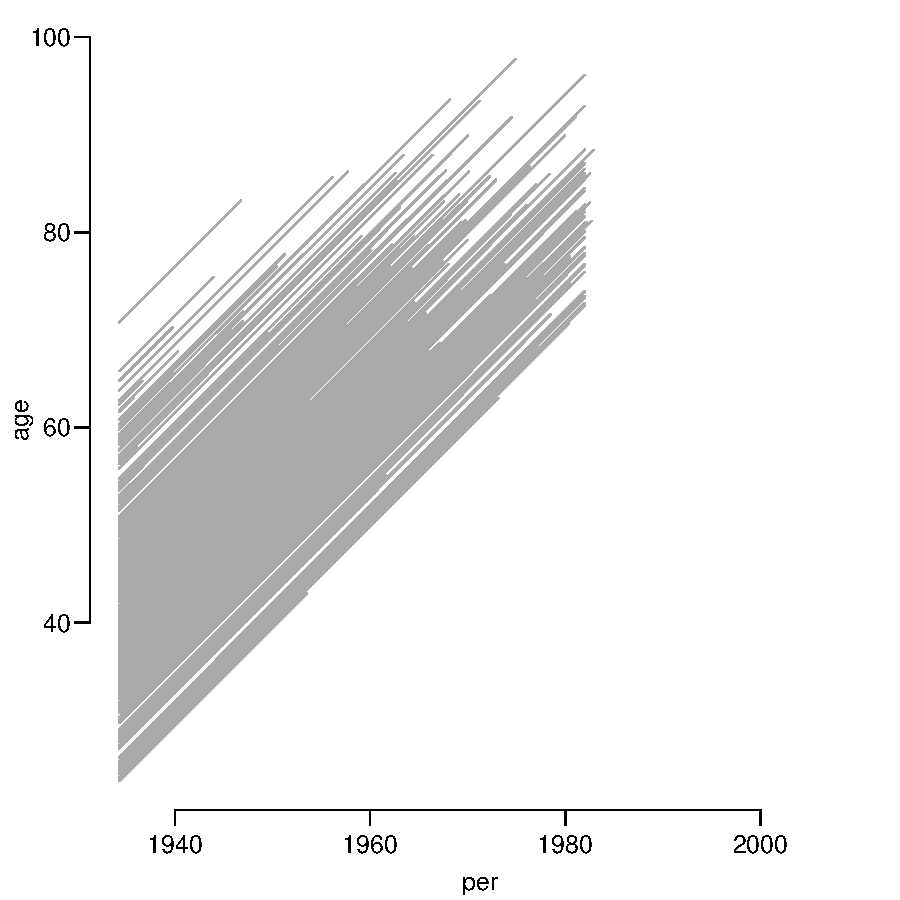
\includegraphics[width=0.39\textwidth]{flup-nicL1}
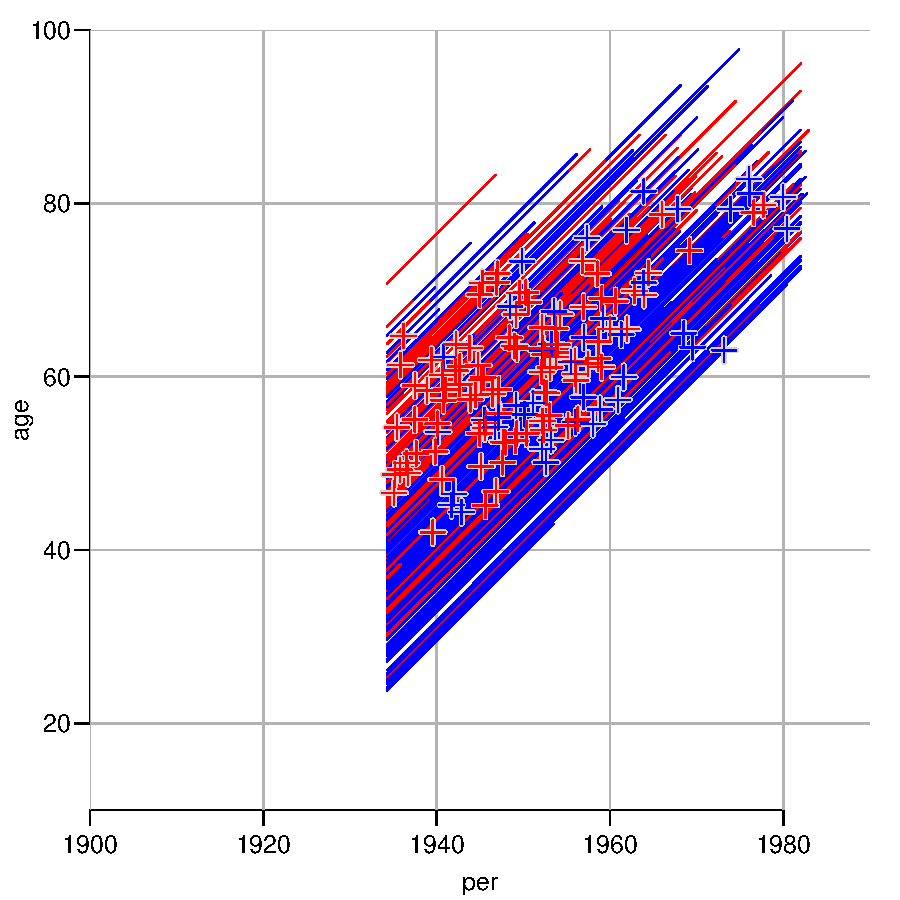
\includegraphics[width=0.59\textwidth]{flup-nicL2}
\caption{\it Lexis diagram of the \textrm{\tt nickel} dataset; left
  panel the default version, right panel with bells and whistles. The
  red lines are for persons with exposure$>0$, so it is pretty evident
  that the oldest ones are the exposed part of the cohort.}
\end{figure}

\chapter{Subdividing follow-up for analysis}

\section{Splitting the follow-up time along a timescale}

The follow-up time in a cohort can be subdivided by for example
current age. This is achieved by the \texttt{splitLexis} (note that it
is \emph{not} called \texttt{split.Lexis}). This requires that the
timescale and the breakpoints on this timescale are supplied. Try:
\begin{Schunk}
\begin{Sinput}
> nicS1 <- splitLexis( nicL, "age", breaks=seq(0,100,10) )
> summary( nicL )
\end{Sinput}
\begin{Soutput}
Transitions:
     To
From   0   1  Records:  Events: Risk time:  Persons:
   0 542 137       679      137   15348.06       679
\end{Soutput}
\begin{Sinput}
> summary( nicS1 )
\end{Sinput}
\begin{Soutput}
Transitions:
     To
From    0   1  Records:  Events: Risk time:  Persons:
   0 2073 137      2210      137   15348.06       679
\end{Soutput}
\end{Schunk}
So we see that the number of events and the amount of follow-up is the
same in the two data sets; only the number of records differ --- the
extra records all have \texttt{lex.Cst}=0 and \texttt{lex.Xst}=0.

To see how records are split for each individual, it is useful to list
the results for a few individuals:
\begin{Schunk}
\begin{Sinput}
> round( subset( nicS1, id %in% 8:10 ), 2 )
\end{Sinput}
\begin{Soutput}
   lex.id     per   age   tfh lex.dur lex.Cst lex.Xst id icd exposure     dob age1st
11      4 1934.25 47.91 23.19    2.09       0       0  8 527        9 1886.34  24.72
12      4 1936.34 50.00 25.28   10.00       0       0  8 527        9 1886.34  24.72
13      4 1946.34 60.00 35.28    9.68       0       0  8 527        9 1886.34  24.72
14      5 1934.25 54.75 24.79    5.25       0       0  9 150        0 1879.50  29.96
15      5 1939.50 60.00 30.04   10.00       0       0  9 150        0 1879.50  29.96
16      5 1949.50 70.00 40.04    6.84       0       0  9 150        0 1879.50  29.96
17      6 1934.25 44.33 23.04    5.67       0       0 10 163        2 1889.91  21.29
18      6 1939.91 50.00 28.71   10.00       0       0 10 163        2 1889.91  21.29
19      6 1949.91 60.00 38.71    2.54       0       1 10 163        2 1889.91  21.29
   agein ageout
11 47.91  69.68
12 47.91  69.68
13 47.91  69.68
14 54.75  76.84
15 54.75  76.84
16 54.75  76.84
17 44.33  62.54
18 44.33  62.54
19 44.33  62.54
\end{Soutput}
\end{Schunk}
The resulting object, \texttt{nicS1}, is again a \texttt{Lexis}
object, and so follow-up may be split further along another
timescale. Subsequently we list the results for individuals 8, 9 and
10 again:
\begin{Schunk}
\begin{Sinput}
> nicS2 <- splitLexis( nicS1, "tfh", breaks=c(0,1,5,10,20,30,100) )
> round( subset( nicS2, id %in% 8:10 ), 2 )
\end{Sinput}
\begin{Soutput}
   lex.id     per   age   tfh lex.dur lex.Cst lex.Xst id icd exposure     dob age1st
13      4 1934.25 47.91 23.19    2.09       0       0  8 527        9 1886.34  24.72
14      4 1936.34 50.00 25.28    4.72       0       0  8 527        9 1886.34  24.72
15      4 1941.06 54.72 30.00    5.28       0       0  8 527        9 1886.34  24.72
16      4 1946.34 60.00 35.28    9.68       0       0  8 527        9 1886.34  24.72
17      5 1934.25 54.75 24.79    5.21       0       0  9 150        0 1879.50  29.96
18      5 1939.46 59.96 30.00    0.04       0       0  9 150        0 1879.50  29.96
19      5 1939.50 60.00 30.04   10.00       0       0  9 150        0 1879.50  29.96
20      5 1949.50 70.00 40.04    6.84       0       0  9 150        0 1879.50  29.96
21      6 1934.25 44.33 23.04    5.67       0       0 10 163        2 1889.91  21.29
22      6 1939.91 50.00 28.71    1.29       0       0 10 163        2 1889.91  21.29
23      6 1941.20 51.29 30.00    8.71       0       0 10 163        2 1889.91  21.29
24      6 1949.91 60.00 38.71    2.54       0       1 10 163        2 1889.91  21.29
   agein ageout
13 47.91  69.68
14 47.91  69.68
15 47.91  69.68
16 47.91  69.68
17 54.75  76.84
18 54.75  76.84
19 54.75  76.84
20 54.75  76.84
21 44.33  62.54
22 44.33  62.54
23 44.33  62.54
24 44.33  62.54
\end{Soutput}
\end{Schunk}
A more efficient (and more intuitive) way of making this double split
is to use the \texttt{splitMulti} function from the \texttt{popEpi}
package:
\begin{Schunk}
\begin{Sinput}
> library( popEpi )
> nicM <- splitMulti( nicL, age = seq(0,100,10), 
+                           tfh = c(0,1,5,10,20,30,100) )
> summary( nicS2 )
\end{Sinput}
\begin{Soutput}
Transitions:
     To
From    0   1  Records:  Events: Risk time:  Persons:
   0 2992 137      3129      137   15348.06       679
\end{Soutput}
\begin{Sinput}
> summary( nicM )
\end{Sinput}
\begin{Soutput}
Transitions:
     To
From    0   1  Records:  Events: Risk time:  Persons:
   0 2992 137      3129      137   15348.06       679
\end{Soutput}
\end{Schunk}
So we see that the two ways of splitting data yields the same amount of
follow-up, but the results are not identical:
\begin{Schunk}
\begin{Sinput}
> identical( nicS2, nicM )
\end{Sinput}
\begin{Soutput}
[1] FALSE
\end{Soutput}
\begin{Sinput}
> class( nicS2 )
\end{Sinput}
\begin{Soutput}
[1] "Lexis"      "data.frame"
\end{Soutput}
\begin{Sinput}
> class( nicM )
\end{Sinput}
\begin{Soutput}
[1] "Lexis"      "data.table" "data.frame"
\end{Soutput}
\end{Schunk}
As we see, this is because the \texttt{nicM} object also is a
\texttt{data.table} object; the \texttt{splitMulti} uses the
\texttt{data.table} machinery which makes the splitting substantially
faster --- this is of particular interest if you operate on large data
sets ($>1,000,000$ records). 

Thus the recommended way of splitting follow-up time is by
\texttt{splitMulti}. But you should be aware that the result is a
\texttt{data.table} object, which in some circumstances behaves
slightly different from \texttt{data.frame}s. See the manual for
\texttt{data.table}.

\subsection{Time scales as covariates}

If we want to model the effect of these timescale variables on
occurrence rates, we will for each interval use either the value of
the left endpoint in each interval or the middle. There is a function
\texttt{timeBand} which returns either of these:
\begin{Schunk}
\begin{Sinput}
> timeBand( nicM, "age", "middle" )[1:20]
\end{Sinput}
\begin{Soutput}
 [1] 45 45 55 65 75 85 95 45 55 55 65 55 45 55 55 65 55 55 65 75
\end{Soutput}
\begin{Sinput}
> # For nice printing and column labelling use the data.frame() function:
> data.frame( nicS2[,c("lex.id","per","age","tfh","lex.dur")],
+             mid.age=timeBand( nicS2, "age", "middle" ),
+               mid.t=timeBand( nicS2, "tfh", "middle" ),
+              left.t=timeBand( nicS2, "tfh", "left"   ),
+             right.t=timeBand( nicS2, "tfh", "right"  ),
+              fact.t=timeBand( nicS2, "tfh", "factor" ) )[1:20,]
\end{Sinput}
\begin{Soutput}
   lex.id      per     age     tfh lex.dur mid.age mid.t left.t right.t   fact.t
1       1 1934.246 45.2273 27.7465  2.2535      45    25     20      30  (20,30]
2       1 1936.500 47.4808 30.0000  2.5192      45    65     30     100 (30,100]
3       1 1939.019 50.0000 32.5192 10.0000      55    65     30     100 (30,100]
4       1 1949.019 60.0000 42.5192 10.0000      65    65     30     100 (30,100]
5       1 1959.019 70.0000 52.5192 10.0000      75    65     30     100 (30,100]
6       1 1969.019 80.0000 62.5192 10.0000      85    65     30     100 (30,100]
7       1 1979.019 90.0000 72.5192  2.9808      95    65     30     100 (30,100]
8       2 1934.246 48.2684 25.0820  1.7316      45    25     20      30  (20,30]
9       2 1935.978 50.0000 26.8136  3.1864      55    25     20      30  (20,30]
10      2 1939.164 53.1864 30.0000  6.8136      55    65     30     100 (30,100]
11      2 1945.978 60.0000 36.8136  3.2712      65    65     30     100 (30,100]
12      3 1934.246 52.9917 27.7465  1.1727      55    25     20      30  (20,30]
13      4 1934.246 47.9067 23.1861  2.0933      45    25     20      30  (20,30]
14      4 1936.340 50.0000 25.2794  4.7206      55    25     20      30  (20,30]
15      4 1941.060 54.7206 30.0000  5.2794      55    65     30     100 (30,100]
16      4 1946.340 60.0000 35.2794  9.6794      65    65     30     100 (30,100]
17      5 1934.246 54.7465 24.7890  5.2110      55    25     20      30  (20,30]
18      5 1939.457 59.9575 30.0000  0.0425      55    65     30     100 (30,100]
19      5 1939.500 60.0000 30.0425 10.0000      65    65     30     100 (30,100]
20      5 1949.500 70.0000 40.0425  6.8442      75    65     30     100 (30,100]
\end{Soutput}
\end{Schunk}
Note that these are characteristics of the intervals defined by
\texttt{breaks=}, \emph{not} the midpoints nor left or right endpoints
of the actual follow-up intervals (which would be \texttt{tfh} and
\texttt{tfh+lex.dur}, respectively). 

These functions are intended for modeling timescale variables as
factors (categorical variables) in which case the coding must be
independent of the censoring and mortality pattern --- it should only
depend on the chosen grouping of the timescale. Modeling timescales as
\emph{quantitative} should not be based on these codings but directly
on the values of the time-scale variables.

\subsection{Differences between time scales}

The midpoint (as well as the left and right interval endpoint) should
be used with caution if the variable \texttt{age1st} is modeled too;
the age at hire is logically equal to the difference between current
age (\texttt{age}) and time since hire (\texttt{thf}):
\begin{Schunk}
\begin{Sinput}
> summary( (nicS2$age-nicS2$tfh) - nicS2$age1st ) 
\end{Sinput}
\begin{Soutput}
      Min.    1st Qu.     Median       Mean    3rd Qu.       Max. 
-7.105e-15  0.000e+00  0.000e+00  2.214e-17  0.000e+00  7.105e-15 
\end{Soutput}
\end{Schunk}
This calculation refer to the \emph{start} of each interval --- the
time scale variables in the \texttt{Lexis} object. But when using the
middle of the intervals, this relationship is not preserved:
\begin{Schunk}
\begin{Sinput}
> summary( timeBand( nicS2, "age", "middle" ) -
+          timeBand( nicS2, "tfh", "middle" ) - nicS2$age1st )
\end{Sinput}
\begin{Soutput}
   Min. 1st Qu.  Median    Mean 3rd Qu.    Max. 
-39.958 -24.178  -5.103 -10.129   2.575  12.519 
\end{Soutput}
\end{Schunk}
If all three variable are to be included in a model, you must make
sure that the \emph{substantial} relationship between the variables be
maintained. One way is to recompute age at first hire from the two
midpoint variables, but more straightforward would be to use the left
endpoint of the intervals, that is the time scale variables in the
\texttt{Lexis} object.  The latter approach however requires that the
follow-up is split in fairly small chunks.

\section{Cutting follow up time at a specific date}

If we have a recording of the date of a specific event as for example
recovery or relapse, we may classify follow-up time as being before or
after this intermediate event, but it requires that follow-up records
that straddle the event be cut into two record. This is achieved with
the function \texttt{cutLexis}, which takes three arguments: the time
point, the timescale, and the value of the (new) state following the
date.

Now we define the age for the nickel workers where the cumulative
exposure exceeds 50 exposure years:
\begin{Schunk}
\begin{Sinput}
> subset( nicL, id %in% 8:10 )
\end{Sinput}
\begin{Soutput}
       per     age     tfh lex.dur lex.Cst lex.Xst lex.id id icd exposure      dob
4 1934.246 47.9067 23.1861 21.7727       0       0      4  8 527        9 1886.340
5 1934.246 54.7465 24.7890 22.0977       0       0      5  9 150        0 1879.500
6 1934.246 44.3314 23.0437 18.2099       0       1      6 10 163        2 1889.915
   age1st   agein  ageout
4 24.7206 47.9067 69.6794
5 29.9575 54.7465 76.8442
6 21.2877 44.3314 62.5413
\end{Soutput}
\begin{Sinput}
> agehi <- nicL$age1st + 50 / nicL$exposure
> nicC <- cutLexis( data = nicL, 
+                    cut = agehi, 
+              timescale = "age",
+              new.state = 2, 
+       precursor.states = 0 )
> subset( nicC, id %in% 8:10 )
\end{Sinput}
\begin{Soutput}
         per     age     tfh lex.dur lex.Cst lex.Xst lex.id id icd exposure      dob
683 1934.246 47.9067 23.1861 21.7727       2       2      4  8 527        9 1886.340
5   1934.246 54.7465 24.7890 22.0977       0       0      5  9 150        0 1879.500
6   1934.246 44.3314 23.0437  1.9563       0       2      6 10 163        2 1889.915
685 1936.203 46.2877 25.0000 16.2536       2       1      6 10 163        2 1889.915
     age1st   agein  ageout
683 24.7206 47.9067 69.6794
5   29.9575 54.7465 76.8442
6   21.2877 44.3314 62.5413
685 21.2877 44.3314 62.5413
\end{Soutput}
\end{Schunk}
(The \texttt{precursor.states=} argument is explained below).  Note
that individual 6 has had his follow-up split at 25 years since hire
where 50 exposure-years were attained. This could also have been
achieved in the split dataset \texttt{nicS2} instead of \texttt{nicL},
try:
\begin{Schunk}
\begin{Sinput}
> subset( nicS2, id %in% 8:10 )
\end{Sinput}
\begin{Soutput}
   lex.id      per     age     tfh lex.dur lex.Cst lex.Xst id icd exposure      dob
13      4 1934.246 47.9067 23.1861  2.0933       0       0  8 527        9 1886.340
14      4 1936.340 50.0000 25.2794  4.7206       0       0  8 527        9 1886.340
15      4 1941.060 54.7206 30.0000  5.2794       0       0  8 527        9 1886.340
16      4 1946.340 60.0000 35.2794  9.6794       0       0  8 527        9 1886.340
17      5 1934.246 54.7465 24.7890  5.2110       0       0  9 150        0 1879.500
18      5 1939.457 59.9575 30.0000  0.0425       0       0  9 150        0 1879.500
19      5 1939.500 60.0000 30.0425 10.0000       0       0  9 150        0 1879.500
20      5 1949.500 70.0000 40.0425  6.8442       0       0  9 150        0 1879.500
21      6 1934.246 44.3314 23.0437  5.6686       0       0 10 163        2 1889.915
22      6 1939.915 50.0000 28.7123  1.2877       0       0 10 163        2 1889.915
23      6 1941.203 51.2877 30.0000  8.7123       0       0 10 163        2 1889.915
24      6 1949.915 60.0000 38.7123  2.5413       0       1 10 163        2 1889.915
    age1st   agein  ageout
13 24.7206 47.9067 69.6794
14 24.7206 47.9067 69.6794
15 24.7206 47.9067 69.6794
16 24.7206 47.9067 69.6794
17 29.9575 54.7465 76.8442
18 29.9575 54.7465 76.8442
19 29.9575 54.7465 76.8442
20 29.9575 54.7465 76.8442
21 21.2877 44.3314 62.5413
22 21.2877 44.3314 62.5413
23 21.2877 44.3314 62.5413
24 21.2877 44.3314 62.5413
\end{Soutput}
\begin{Sinput}
> agehi <- nicS2$age1st + 50 / nicS2$exposure
> nicS2C <- cutLexis( data = nicS2, 
+                      cut = agehi, 
+                timescale = "age",
+                new.state = 2, 
+         precursor.states = 0 )
> subset( nicS2C, id %in% 8:10 )
\end{Sinput}
\begin{Soutput}
     lex.id      per     age     tfh lex.dur lex.Cst lex.Xst id icd exposure      dob
3142      4 1934.246 47.9067 23.1861  2.0933       2       2  8 527        9 1886.340
3143      4 1936.340 50.0000 25.2794  4.7206       2       2  8 527        9 1886.340
3144      4 1941.060 54.7206 30.0000  5.2794       2       2  8 527        9 1886.340
3145      4 1946.340 60.0000 35.2794  9.6794       2       2  8 527        9 1886.340
17        5 1934.246 54.7465 24.7890  5.2110       0       0  9 150        0 1879.500
18        5 1939.457 59.9575 30.0000  0.0425       0       0  9 150        0 1879.500
19        5 1939.500 60.0000 30.0425 10.0000       0       0  9 150        0 1879.500
20        5 1949.500 70.0000 40.0425  6.8442       0       0  9 150        0 1879.500
21        6 1934.246 44.3314 23.0437  1.9563       0       2 10 163        2 1889.915
3150      6 1936.203 46.2877 25.0000  3.7123       2       2 10 163        2 1889.915
3151      6 1939.915 50.0000 28.7123  1.2877       2       2 10 163        2 1889.915
3152      6 1941.203 51.2877 30.0000  8.7123       2       2 10 163        2 1889.915
3153      6 1949.915 60.0000 38.7123  2.5413       2       1 10 163        2 1889.915
      age1st   agein  ageout
3142 24.7206 47.9067 69.6794
3143 24.7206 47.9067 69.6794
3144 24.7206 47.9067 69.6794
3145 24.7206 47.9067 69.6794
17   29.9575 54.7465 76.8442
18   29.9575 54.7465 76.8442
19   29.9575 54.7465 76.8442
20   29.9575 54.7465 76.8442
21   21.2877 44.3314 62.5413
3150 21.2877 44.3314 62.5413
3151 21.2877 44.3314 62.5413
3152 21.2877 44.3314 62.5413
3153 21.2877 44.3314 62.5413
\end{Soutput}
\end{Schunk}
The same results would have emerged if we had used the \texttt{nicM}
dataset (the \texttt{data.table} object). Mathematicians would say
that \texttt{splitLexis} and \texttt{cutLexis} are commutative.

Note that follow-up subsequent to the event is classified as being in
state 2, but that the final transition to state 1 (death from lung
cancer) is preserved. This is the point of the
\texttt{precursor.states=} argument. It names the states (in this case
0, ``Alive'') that will be over-written by \texttt{new.state} (in this
case state 2, ``High exposure''), while state 1 (``Dead'') should not
be updated even if it is after the time where the persons moves to
state 2. In other words, only state 0 is a precursor to state 2, state
1 is always subsequent to state 2. Even if you at a high exposure
level, death is pretty final.

If the intermediate event is to be used as a time-dependent variable
in a Cox-model, then \texttt{lex.Cst} should be used as the
time-dependent variable, and \texttt{lex.Xst==1} as the event.

\chapter{Modeling rates}

\section{Background}

The purpose of subdividing follow-up data is to be able to model the
effects of the time scale variables as parametric functions. 

In a model that assumes a constant occurrence rate in each of the
intervals the likelihood contribution from each interval is the same
as the likelihood contribution from a Poisson variate $D$, say, with
mean $\lambda\ell$ where $\lambda$ is the rate and $\ell$ is the
interval length, and where the value of the variate $D$ is 1 or 0
according to whether an event has occurred or not. Moreover, the
likelihood contributions from all follow-up intervals from a single
person are \emph{conditionally} independent (conditional on having
survived till the start of the interval in question). This implies
that the total contribution to the likelihood from a single person is
a product of terms, and hence the same as the likelihood of a number
of independent Poisson terms, one from each interval.

Parametric modeling of the rates is obtained by using the \emph{value}
of the timescale for each interval as quantitative explanatory
variables, using for example splines. Thus the model will be one where
the rate is assumed constant in each interval, but where a parametric
form of the \emph{size} of the rate in each interval is imposed by the
model, using the timescale as a covariate.

\section{Practicalities}

In the nickel worker study we might want to look at the effects of age
and time since hire. If we want to use splines we must allocate knots
for anchoring the splines at each of the time scales, either by some
\textit{ad hoc} method or by using some sort of penalized splines. The
letter will not be treated here.

Here we shall use the former approach and allocate 5 knots on each of
the two time-scales. We allocate knots so that we have the event evenly
distributed between the knots:
\begin{Schunk}
\begin{Sinput}
> ( a.kn <- with( subset( nicM, lex.Xst==1 ), quantile( age+lex.dur, (1:5-0.5)/5 ) ) )
\end{Sinput}
\begin{Soutput}
     10%      30%      50%      70%      90% 
50.11874 55.61674 61.09590 64.88704 73.32220 
\end{Soutput}
\begin{Sinput}
> ( t.kn <- with( subset( nicM, lex.Xst==1 ), quantile( tfh+lex.dur, (1:5-0.5)/5 ) ) )
\end{Sinput}
\begin{Soutput}
     10%      30%      50%      70%      90% 
24.25572 30.02202 34.00440 39.84592 45.95512 
\end{Soutput}
\end{Schunk}
In the \texttt{Epi} package there is a convenience wrapper for the
\texttt{n}atural \texttt{s}pline generator \texttt{ns}, \texttt{Ns},
that takes the smallest and the largest of a set of supplied knots to
be the boundary knots.

\section{Models for rates}

\subsection{One time scale}

A model that only models lung cancer mortality
rates as a function of age would then be:
\begin{Schunk}
\begin{Sinput}
> ma <- glm( (lex.Xst==1) ~ Ns(age,knots=a.kn),
+            family = poisson,
+            offset = log(lex.dur),
+              data = nicM )
> summary( ma )
\end{Sinput}
\begin{Soutput}
Call:
glm(formula = (lex.Xst == 1) ~ Ns(age, knots = a.kn), family = poisson, 
    data = nicM, offset = log(lex.dur))

Deviance Residuals: 
    Min       1Q   Median       3Q      Max  
-0.5074  -0.3896  -0.2143  -0.1203   3.7904  

Coefficients:
                       Estimate Std. Error z value Pr(>|z|)
(Intercept)             -4.6591     0.1324 -35.199  < 2e-16
Ns(age, knots = a.kn)1   0.1671     0.2970   0.563  0.57371
Ns(age, knots = a.kn)2  -0.1315     0.3727  -0.353  0.72411
Ns(age, knots = a.kn)3   0.7827     0.2885   2.713  0.00667
Ns(age, knots = a.kn)4  -0.3717     0.2780  -1.337  0.18125

(Dispersion parameter for poisson family taken to be 1)

    Null deviance: 1024.38  on 3128  degrees of freedom
Residual deviance:  979.16  on 3124  degrees of freedom
AIC: 1263.2

Number of Fisher Scoring iterations: 7
\end{Soutput}
\end{Schunk}
The offset, \texttt{log(lex.dur)} comes from the fact that the
likelihood for the follow-up data is the same as that for independent
Poisson variates with mean $\lambda\ell$, and that the default link
function for the Poisson family is the log, so that we are using a
linear model for the log-mean, that is $\log(\lambda) + \log(\ell)$.
But when we want a model for the log-rate ($\log(\lambda)$), the term
$\log(\ell)$ must be included as a covariate with regression
coefficient fixed to 1; a so-called offset.

The parameters from the model do not have any direct interpretation
\textit{per se}, but we can compute the estimated lung cancer incidence
rates for a range of ages using \texttt{ci.pred} with a suitably
defined prediction data frame. Note that we must specify all
covariates in the model, also the variable in the offset,
\texttt{lex.dur}. We set the latter to 1000, because we want the lung
cancer mortality rates per 1000 PY. By default \texttt{ci.pred} yields a
prediction on the response-scale, that is the rate-scale:
\begin{Schunk}
\begin{Sinput}
> nd <- data.frame( age=40:85, lex.dur=1000 )
> pr.a <- ci.pred( ma, newdata = nd )
> matplot( nd$age, pr.a,
+          type="l", lty=1, col=1, lwd=c(3,1,1),
+          log="y", xlab="Age (years)",
+          ylab="Lunng cancer mortality per 1000 PY")
\end{Sinput}
\end{Schunk}
\insfig{pr-a}{0.8}{Lung cancer mortality among Nickel smelter workers
  by age. We see that the rates increase till about 55 years, and from
then on is approximately flat.}

\subsection{More time scales}

There may however also be an effect of time since hire too, so we can
add this term to the model:
\begin{Schunk}
\begin{Sinput}
> mat <- update( ma, . ~ . + Ns(tfh,knots=t.kn) )
> summary( mat )
\end{Sinput}
\begin{Soutput}
Call:
glm(formula = (lex.Xst == 1) ~ Ns(age, knots = a.kn) + Ns(tfh, 
    knots = t.kn), family = poisson, data = nicM, offset = log(lex.dur))

Deviance Residuals: 
    Min       1Q   Median       3Q      Max  
-0.6308  -0.3730  -0.2170  -0.1180   3.8903  

Coefficients:
                       Estimate Std. Error z value Pr(>|z|)
(Intercept)            -4.65125    0.14844 -31.335   <2e-16
Ns(age, knots = a.kn)1  0.19029    0.32601   0.584   0.5594
Ns(age, knots = a.kn)2  0.04239    0.40857   0.104   0.9174
Ns(age, knots = a.kn)3  0.87848    0.37395   2.349   0.0188
Ns(age, knots = a.kn)4  0.08124    0.37567   0.216   0.8288
Ns(tfh, knots = t.kn)1  0.05961    0.45702   0.130   0.8962
Ns(tfh, knots = t.kn)2 -0.30254    0.39214  -0.771   0.4404
Ns(tfh, knots = t.kn)3 -0.08144    0.37493  -0.217   0.8281
Ns(tfh, knots = t.kn)4 -0.63400    0.34055  -1.862   0.0626

(Dispersion parameter for poisson family taken to be 1)

    Null deviance: 1024.4  on 3128  degrees of freedom
Residual deviance:  970.7  on 3120  degrees of freedom
AIC: 1262.7

Number of Fisher Scoring iterations: 7
\end{Soutput}
\end{Schunk}
This model has two time scales, age and time since hire, so it makes
little sense to report the effect of age for a \emph{fixed} value of
time since hire --- the time since hire increases by age.
Instead we can show the mortality rates for persons hired at different
ages, and report the \emph{joint} effect of increasing age and time
since hire.

In order to get a feeling for the values that can be use we look at \texttt{age1st}
\begin{Schunk}
\begin{Sinput}
> summary( nickel$age1st )
\end{Sinput}
\begin{Soutput}
   Min. 1st Qu.  Median    Mean 3rd Qu.    Max. 
  10.78   21.80   26.16   26.74   30.63   52.19 
\end{Soutput}
\end{Schunk}
Thus we shall show mortality rates in ages 20--90 for persons hired in
ages 15, 25, 35 and 45:
\begin{Schunk}
\begin{Sinput}
> nd <- data.frame( expand.grid( age=c(20:90,NA), age1st=seq(15,45,10) ) ) 
> nd <- transform( nd, tfh = ifelse( age > age1st, age-age1st, NA ),
+                  lex.dur = 1000 )
> # makes no sense to have age < age1st
> nd <- transform( nd, age = ifelse( age > age1st, age, NA ) )
> head( nd )
\end{Sinput}
\begin{Soutput}
  age age1st tfh lex.dur
1  20     15   5    1000
2  21     15   6    1000
3  22     15   7    1000
4  23     15   8    1000
5  24     15   9    1000
6  25     15  10    1000
\end{Soutput}
\end{Schunk}
With this in place we can plot the estimated rates as before, only
now we will get 4 separate lines. The purpose of inserting an
\texttt{NA} on the age-scale in the \texttt{expand.grid} is that the
different instances of \texttt{age1st} be separated by \texttt{NA}s, and
hence will not be connected when we plot the curves. The downside of
this trick is that lines cannot be plotted with different colors or
symbols.
\begin{Schunk}
\begin{Sinput}
> pr.at <- ci.pred( mat, newdata = nd )
> matplot( nd$age, pr.at,
+          type="l", lty=1, col=1, lwd=c(3,1,1),
+          log="y", xlab="Age (years)",
+          ylab="Lunng cancer mortality per 1000 PY")
\end{Sinput}
\end{Schunk}
\insfig{pr-at}{0.8}{Lung cancer mortality among Nickel smelter workers
  by age and age at hire 15, 25,35 and 45. Each line (except the
  first) starts at the age of hire; we see that the later in life you
  are hired, the smaller the initial risk, but the higher the eventual
  risk of lung cancer death.}

We can check whether the effect of time since hire is actually
improving the model:
\begin{Schunk}
\begin{Sinput}
> anova( ma, mat, test="Chisq" )
\end{Sinput}
\begin{Soutput}
Analysis of Deviance Table

Model 1: (lex.Xst == 1) ~ Ns(age, knots = a.kn)
Model 2: (lex.Xst == 1) ~ Ns(age, knots = a.kn) + Ns(tfh, knots = t.kn)
  Resid. Df Resid. Dev Df Deviance Pr(>Chi)
1      3124     979.16                     
2      3120     970.70  4   8.4626  0.07603
\end{Soutput}
\end{Schunk}
We see a pretty strong indication that this is the case.

\subsection{Difference between time scales}

However it might be the case that it really is the age at first hire
that is the main determinant (recall that
$\mathtt{age}-\mathtt{thf}=\mathtt{age1st}$), so we could fit a model
with this variable instead --- a model with only 1 timescale, namely
\texttt{age}.
\begin{Schunk}
\begin{Sinput}
> ( f.kn <- with( subset( nicM, lex.Xst==1 ), quantile( age1st, (1:5-0.5)/5 ) ) )
\end{Sinput}
\begin{Soutput}
     10%      30%      50%      70%      90% 
20.25860 22.55422 26.00000 28.36578 33.96910 
\end{Soutput}
\begin{Sinput}
> maf <- update( ma, . ~ . + Ns(age1st,knots=f.kn) )
> summary( maf )
\end{Sinput}
\begin{Soutput}
Call:
glm(formula = (lex.Xst == 1) ~ Ns(age, knots = a.kn) + Ns(age1st, 
    knots = f.kn), family = poisson, data = nicM, offset = log(lex.dur))

Deviance Residuals: 
    Min       1Q   Median       3Q      Max  
-0.5696  -0.3671  -0.2257  -0.1197   3.7777  

Coefficients:
                          Estimate Std. Error z value Pr(>|z|)
(Intercept)               -4.62646    0.17564 -26.340  < 2e-16
Ns(age, knots = a.kn)1     0.21589    0.29742   0.726  0.46792
Ns(age, knots = a.kn)2    -0.06427    0.37653  -0.171  0.86446
Ns(age, knots = a.kn)3     0.79456    0.29345   2.708  0.00678
Ns(age, knots = a.kn)4    -0.31305    0.27976  -1.119  0.26314
Ns(age1st, knots = f.kn)1 -0.15145    0.38279  -0.396  0.69237
Ns(age1st, knots = f.kn)2  0.04607    0.27980   0.165  0.86923
Ns(age1st, knots = f.kn)3  0.26374    0.26156   1.008  0.31331
Ns(age1st, knots = f.kn)4 -0.22878    0.23117  -0.990  0.32234

(Dispersion parameter for poisson family taken to be 1)

    Null deviance: 1024.4  on 3128  degrees of freedom
Residual deviance:  973.2  on 3120  degrees of freedom
AIC: 1265.2

Number of Fisher Scoring iterations: 7
\end{Soutput}
\begin{Sinput}
> anova( maf, ma, mat, test="Chisq" )
\end{Sinput}
\begin{Soutput}
Analysis of Deviance Table

Model 1: (lex.Xst == 1) ~ Ns(age, knots = a.kn) + Ns(age1st, knots = f.kn)
Model 2: (lex.Xst == 1) ~ Ns(age, knots = a.kn)
Model 3: (lex.Xst == 1) ~ Ns(age, knots = a.kn) + Ns(tfh, knots = t.kn)
  Resid. Df Resid. Dev Df Deviance Pr(>Chi)
1      3120     973.20                     
2      3124     979.16 -4  -5.9624  0.20198
3      3120     970.70  4   8.4626  0.07603
\end{Soutput}
\end{Schunk}
We see that there is much less indication that the age at first hire has
an effect.

For the sake of completeness we can draw the predicted values from the
\texttt{maf} model on top of the ones from the \textrm{mat} model:
\begin{Schunk}
\begin{Sinput}
> pr.af <- ci.pred( maf, newdata = nd )
> matplot( nd$age, pr.at,
+          type="l", lty=1, col=1, lwd=c(3,1,1),
+          log="y", xlab="Age (years)",
+          ylab="Lunng cancer mortality per 1000 PY")
> matlines( nd$age, pr.af,
+          type="l", lty=1, col=2, lwd=c(3,0,0) )
\end{Sinput}
\end{Schunk}
\insfig{pr-at-af}{0.8}{Lung cancer mortality among Nickel smelter
  workers by age and age at hire 15, 25,35 and 45. Each line (except
  the first) starts at the age of hire; we see that the later in life
  you are hired, the smaller the initial risk, but the higher the
  eventual risk of lung cancer death. The red lines are from the model
  \textrm{\tt maf} where the lines are constrained to be parallel, and
  which gives a worse fit to data.}

\subsection{The complete picture --- exercise}

We could fit the remaining models where one or more of the three
variables are included, and compare all of them:
\begin{Schunk}
\begin{Sinput}
> maft <- update( mat, . ~ . + Ns(age1st,knots=f.kn) )
> summary( maft )
\end{Sinput}
\begin{Soutput}
Call:
glm(formula = (lex.Xst == 1) ~ Ns(age, knots = a.kn) + Ns(tfh, 
    knots = t.kn) + Ns(age1st, knots = f.kn), family = poisson, 
    data = nicM, offset = log(lex.dur))

Deviance Residuals: 
    Min       1Q   Median       3Q      Max  
-0.5899  -0.3579  -0.2224  -0.1185   3.8687  

Coefficients: (1 not defined because of singularities)
                          Estimate Std. Error z value Pr(>|z|)
(Intercept)               -4.71537    0.16481 -28.612   <2e-16
Ns(age, knots = a.kn)1     0.01671    0.35152   0.048   0.9621
Ns(age, knots = a.kn)2    -0.11682    0.44638  -0.262   0.7935
Ns(age, knots = a.kn)3     0.47689    0.50638   0.942   0.3463
Ns(age, knots = a.kn)4    -0.18241    0.47318  -0.385   0.6999
Ns(tfh, knots = t.kn)1     0.35272    0.51329   0.687   0.4920
Ns(tfh, knots = t.kn)2    -0.11034    0.43043  -0.256   0.7977
Ns(tfh, knots = t.kn)3     0.26874    0.49133   0.547   0.5844
Ns(tfh, knots = t.kn)4    -0.30302    0.43585  -0.695   0.4869
Ns(age1st, knots = f.kn)1 -0.10650    0.37476  -0.284   0.7763
Ns(age1st, knots = f.kn)2  0.17245    0.20063   0.860   0.3900
Ns(age1st, knots = f.kn)3  0.47357    0.24239   1.954   0.0507
Ns(age1st, knots = f.kn)4       NA         NA      NA       NA

(Dispersion parameter for poisson family taken to be 1)

    Null deviance: 1024.38  on 3128  degrees of freedom
Residual deviance:  966.31  on 3117  degrees of freedom
AIC: 1264.3

Number of Fisher Scoring iterations: 7
\end{Soutput}
\begin{Sinput}
> mft <- update( maft, . ~ . - Ns(age,knots=a.kn) )
> mf  <- update( maf , . ~ . - Ns(age,knots=a.kn) )
> mt  <- update( mat , . ~ . - Ns(age,knots=a.kn) )
> allp <- anova( maft, mat, ma, maf, mf, mft, mt, mat,
+                maf, maft, mft,
+                test="Chisq" )
> mall <- as.matrix( allp )
> cbind( mod = c("maft","mat","ma","maf","mf","mft","mt","mat","maf","maft","mft"),
+        round( allp[,1:5], 3 ) )
\end{Sinput}
\begin{Soutput}
    mod Resid. Df Resid. Dev Df Deviance Pr(>Chi)
1  maft      3117    966.306 NA       NA       NA
2   mat      3120    970.697 -3   -4.391    0.222
3    ma      3124    979.160 -4   -8.463    0.076
4   maf      3120    973.197  4    5.962    0.202
5    mf      3124   1011.593 -4  -38.396    0.000
6   mft      3120    971.120  4   40.473    0.000
7    mt      3124    985.734 -4  -14.614    0.006
8   mat      3120    970.697  4   15.037    0.005
9   maf      3120    973.197  0   -2.500       NA
10 maft      3117    966.306  3    6.892    0.075
11  mft      3120    971.120 -3   -4.814    0.186
\end{Soutput}
\end{Schunk}
\begin{enumerate}
\item Explain why there are \texttt{NA}s among the parameters in the
  model \texttt{maf}.
\item Draw a graph (a ``DAG'') with the models as nodes and the tests
  as vertices, put the p-values on the vertices and use the result to
  argue that the model with age an time since hire is actually the
  most sensible description in this case.
\end{enumerate}

\chapter{Competing risks --- multiple types of events}

If we want to consider death from lung cancer and death from other
causes as separate events we can code these as for example 1 and 2.
\begin{Schunk}
\begin{Sinput}
> data( nickel )
> nicL <- Lexis( entry = list( per = agein+dob,
+                              age = agein,
+                              tfh = agein-age1st ),
+                 exit = list( age = ageout ),
+          exit.status = ( icd > 0 ) + ( icd %in% c(162,163) ),
+                 data = nickel )
\end{Sinput}
\begin{Soutput}
NOTE: entry.status has been set to 0 for all.
\end{Soutput}
\begin{Sinput}
> summary( nicL )
\end{Sinput}
\begin{Soutput}
Transitions:
     To
From  0   1   2  Records:  Events: Risk time:  Persons:
   0 47 495 137       679      632   15348.06       679
\end{Soutput}
\begin{Sinput}
> subset( nicL, id %in% 8:10 )
\end{Sinput}
\begin{Soutput}
       per     age     tfh lex.dur lex.Cst lex.Xst lex.id id icd exposure      dob
4 1934.246 47.9067 23.1861 21.7727       0       1      4  8 527        9 1886.340
5 1934.246 54.7465 24.7890 22.0977       0       1      5  9 150        0 1879.500
6 1934.246 44.3314 23.0437 18.2099       0       2      6 10 163        2 1889.915
   age1st   agein  ageout
4 24.7206 47.9067 69.6794
5 29.9575 54.7465 76.8442
6 21.2877 44.3314 62.5413
\end{Soutput}
\end{Schunk}
In order to have a more readable output we can label the states, we
can enter the names of these in the \texttt{states} parameter, try for
example:
\begin{Schunk}
\begin{Sinput}
> nicL <- Lexis( entry = list( per = agein+dob,
+                              age = agein,
+                              tfh = agein-age1st ),
+                 exit = list( age = ageout ),
+          exit.status = ( icd > 0 ) + ( icd %in% c(162,163) ),
+                 data = nickel,
+               states = c("Alive","D.oth","D.lung") )
\end{Sinput}
\begin{Soutput}
NOTE: entry.status has been set to 0 for all.
\end{Soutput}
\begin{Sinput}
> summary( nicL )
\end{Sinput}
\begin{Soutput}
Transitions:
     To
From    Alive D.oth D.lung  Records:  Events: Risk time:  Persons:
  Alive    47   495    137       679      632   15348.06       679
\end{Soutput}
\begin{Sinput}
> str( nicL )
\end{Sinput}
\begin{Soutput}
Classes ‘Lexis’ and 'data.frame':	679 obs. of  14 variables:
 $ per     : num  1934 1934 1934 1934 1934 ...
 $ age     : num  45.2 48.3 53 47.9 54.7 ...
 $ tfh     : num  27.7 25.1 27.7 23.2 24.8 ...
 $ lex.dur : num  47.75 15 1.17 21.77 22.1 ...
 $ lex.Cst : Factor w/ 3 levels "Alive","D.oth",..: 1 1 1 1 1 1 1 1 1 1 ...
 $ lex.Xst : Factor w/ 3 levels "Alive","D.oth",..: 1 3 3 2 2 3 2 2 2 2 ...
 $ lex.id  : int  1 2 3 4 5 6 7 8 9 10 ...
 $ id      : num  3 4 6 8 9 10 15 16 17 18 ...
 $ icd     : num  0 162 163 527 150 163 334 160 420 12 ...
 $ exposure: num  5 5 10 9 0 2 0 0.5 0 0 ...
 $ dob     : num  1889 1886 1881 1886 1880 ...
 $ age1st  : num  17.5 23.2 25.2 24.7 30 ...
 $ agein   : num  45.2 48.3 53 47.9 54.7 ...
 $ ageout  : num  93 63.3 54.2 69.7 76.8 ...
 - attr(*, "time.scales")= chr  "per" "age" "tfh"
 - attr(*, "time.since")= chr  "" "" ""
 - attr(*, "breaks")=List of 3
  ..$ per: NULL
  ..$ age: NULL
  ..$ tfh: NULL
\end{Soutput}
\end{Schunk}
Note that the \texttt{Lexis} function automatically assumes that all
persons enter in the first level (given in the \texttt{states=}
argument), corresponding to the numerical values given in
\texttt{exit.status}.

When we cut at a date as in this case, the date where cumulative
exposure exceeds 50 exposure-years, we get the follow-up \emph{after}
the date classified as being in the new state if the exit
(\texttt{lex.Xst}) was to a state we defined as one of the
\texttt{precursor.states}:
\begin{Schunk}
\begin{Sinput}
> nicL$agehi <- nicL$age1st + 50 / nicL$exposure
> nicC <- cutLexis( data = nicL,
+                    cut = nicL$agehi,
+              timescale = "age",
+              new.state = "HiExp",
+       precursor.states = "Alive" )
> subset( nicC, id %in% 8:10 )
\end{Sinput}
\begin{Soutput}
         per     age     tfh lex.dur lex.Cst lex.Xst lex.id id icd exposure      dob
683 1934.246 47.9067 23.1861 21.7727   HiExp   D.oth      4  8 527        9 1886.340
5   1934.246 54.7465 24.7890 22.0977   Alive   D.oth      5  9 150        0 1879.500
6   1934.246 44.3314 23.0437  1.9563   Alive   HiExp      6 10 163        2 1889.915
685 1936.203 46.2877 25.0000 16.2536   HiExp  D.lung      6 10 163        2 1889.915
     age1st   agein  ageout    agehi
683 24.7206 47.9067 69.6794 30.27616
5   29.9575 54.7465 76.8442      Inf
6   21.2877 44.3314 62.5413 46.28770
685 21.2877 44.3314 62.5413 46.28770
\end{Soutput}
\begin{Sinput}
> summary( nicC, scale=1000 )
\end{Sinput}
\begin{Soutput}
Transitions:
     To
From    Alive HiExp D.oth D.lung  Records:  Events: Risk time:  Persons:
  Alive    39    83   279     65       466      427      10.77       466
  HiExp     0     8   216     72       296      288       4.58       296
  Sum      39    91   495    137       762      715      15.35       679
\end{Soutput}
\end{Schunk}
Note that the persons-years is the same, but that the number of
events has changed. This is because events are now defined as any
transition, including the transitions to \texttt{HiExp}.

Also note that (so far) it is necessary to specify the variable with
the cut points in full, using only \texttt{cut=agehi} would give an error.

\section{Subdividing states}

It may be of interest to subdivide the states following the
intermediate event according to whether the event has occurred or
not. That is done by the argument \texttt{split.states=TRUE}.

Moreover, it will also often be of interest to introduce a new
timescale indicating the time since intermediate event. This can be
done by the argument \texttt{new.scale=TRUE}, alternatively
\texttt{new.scale="tfe"}, as illustrated here:
\begin{Schunk}
\begin{Sinput}
> nicC <- cutLexis( data = nicL,
+                    cut = nicL$agehi,
+              timescale = "age",
+              new.state = "HiExp",
+              new.scale = "tfe",
+           split.states = TRUE,
+       precursor.states = "Alive" )
> subset( nicC, id %in% 8:10 )
\end{Sinput}
\begin{Soutput}
         per     age     tfh      tfe lex.dur lex.Cst       lex.Xst lex.id id icd
683 1934.246 47.9067 23.1861 17.63054 21.7727   HiExp  D.oth(HiExp)      4  8 527
5   1934.246 54.7465 24.7890       NA 22.0977   Alive         D.oth      5  9 150
6   1934.246 44.3314 23.0437       NA  1.9563   Alive         HiExp      6 10 163
685 1936.203 46.2877 25.0000  0.00000 16.2536   HiExp D.lung(HiExp)      6 10 163
    exposure      dob  age1st   agein  ageout    agehi
683        9 1886.340 24.7206 47.9067 69.6794 30.27616
5          0 1879.500 29.9575 54.7465 76.8442      Inf
6          2 1889.915 21.2877 44.3314 62.5413 46.28770
685        2 1889.915 21.2877 44.3314 62.5413 46.28770
\end{Soutput}
\begin{Sinput}
> summary( nicC, scale=1000, timeScales=TRUE )
\end{Sinput}
\begin{Soutput}
Transitions:
     To
From    Alive HiExp D.oth D.lung D.lung(HiExp) D.oth(HiExp)  Records:  Events: Risk time:
  Alive    39    83   279     65             0            0       466      427      10.77
  HiExp     0     8     0      0            72          216       296      288       4.58
  Sum      39    91   279     65            72          216       762      715      15.35
       
Transitions:
     To
From     Persons:
  Alive       466
  HiExp       296
  Sum         679

Timescales:
  time.scale time.since
1        per           
2        age           
3        tfh           
4        tfe      HiExp
\end{Soutput}
\end{Schunk}
Note that the \texttt{timeScales=TRUE} to \texttt{summary} lists the
timescales available in the object, and also indicates which of them
that are defined as time since entry to a particular state. This
facility is not used here, but it is needed when simulating follow-up
data --- see the vignette on \textrm{simLexis}.

With 6 different states it is quite difficult to get an overview of
the transitions between states from the \texttt{summary()}. Therefore
there is function that gives a graphical display of the states showing
the transitions between the states:
\begin{Schunk}
\begin{Sinput}
> boxes( nicC, boxpos = list(x=c(10,10,80,80,80,80),
+                            y=c(75,25,87,63,13,37)),
+             scale.Y = 1000,
+             show.BE = TRUE )
\end{Sinput}
\end{Schunk}
\insfig{nic-box}{0.9}{Transitions between states; the number in the
  middle of each box is the person-years (in 1000s --- since
  \textrm{\tt scale.Y=1000}), the numbers at the bottom of the boxes
  are the number that start, respectively end their follow-up in each
  state.  The numbers on the arrows are the number of transitions and
  crude transition rates (the latter in events per 1000 PY).\newline
  The function \textrm{\tt boxes.Lexis} has a zillion arguments to
  fine-tune the appearance of the display in terms of colors etc.}

%% \section{Multiple events of the same type (recurrent events)}
%% Sometimes more events of the same type are recorded for each person and
%% one would then like to count these and put follow-up time in states accordingly.
%% Essentially, each set of cutpoints represents progressions from one
%% state to the next. Therefore the states should be numbered, and the
%% numbering of states subsequently occupied be increased accordingly.

%% This is a behaviour different from the one outlined above, and it is
%% achieved by the argument \texttt{count=TRUE} to
%% \texttt{cutLexis}. When \texttt{count} is set to \texttt{TRUE}, the
%% value of the arguments \texttt{new.state} and
%% \texttt{precursor.states} are ignored.  Actually, when using the
%% argument \texttt{count=TRUE}, the function \texttt{countLexis} is
%% called, so an alternative is to use this directly.

%% \renewcommand{\bibname}{References}
%% \bibliographystyle{plain}
%% \bibliography{%
%% /home/bendix/art/bibtex/BxC,%
%% /home/bendix/art/bibtex/Stat,%
%% /home/bendix/art/bibtex/DMCa,%
%% /home/bendix/art/bibtex/Diabetes%
%% }
%% \addcontentsline{toc}{section}{\bibname}

\end{document}
